\shorthandoff{:!} %règle un problème de compatibilité avec babel
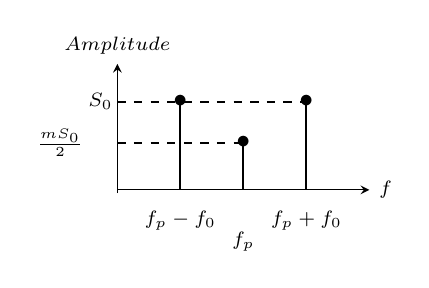
\begin{tikzpicture}[scale=0.40]
	
	%axes
	\draw[->,>=stealth] (0,0) -- (8,0) node[right] {\scriptsize{$f$}};
	%
	\draw[->,>=stealth] (0,-0.1) -- (0,4)node[above] {\scriptsize{$Amplitude$}};

	% spectres 
	%%% raies 
	\draw [color=black,thick, smooth, samples=150] (4,0) -- (4,1.5)node[midway,below=20pt] {\scriptsize{$f_p$}};
	\draw (4,1.5) node {$\bullet$};
	\draw [color=black,thick, smooth, samples=150] (2,0) -- (2,2.8)node[midway,below=20pt] {\scriptsize{$f_p-f_0$}};
	\draw (2,2.8) node {$\bullet$};
	\draw [color=black,thick, smooth, samples=150] (6,0) -- (6,2.8)node[midway,below=20pt] {\scriptsize{$f_p+f_0$}};
	\draw (6,2.8) node {$\bullet$};
	%%%  amplitudes des raies
	\draw [color=black,thick, dashed, samples=150] (0,2.8) -- (6,2.8)node[near start, left=15pt] {\scriptsize{$S_0$}};
	\draw [color=black,thick, dashed, samples=150] (0,1.5) -- (4,1.5)node[near start, left=20pt] {\scriptsize{$\frac{m S_0}{2}$}};
\end{tikzpicture} 
\shorthandon{:!}